%---------- Segundo Capitulo ----------
\chapter{Fundamentação Teórica}
Em sistemas computacionais em que a identificação e autenticação do usuário são premissas na segurança de transações e processos, é interessante manter mecanismos que ofereçam aos usuários, meios confiáveis no estabelecimento dessas conexões.
\begin{citacao}
Durante as primeiras décadas de sua existência, as redes de computadores foram usadas principalmente por pesquisadores universitários, com a finalidade de enviar mensagens de correio eletrônico, e também por funcionários de empresas, para compartilhar impressoras. Sob essas condições, a segurança nunca precisou de maiores cuidados. Porém, como milhões de cidadãos comuns atualmente estão usando as redes para executar operações bancárias, fazer compras e arquivar sua devolução de impostos, a segurança das redes está despontando no horizonte como um problema potencial.\cite{tanenbaum2003redes}
\end{citacao}
Frequentemente para utilizar algum recurso computacional são utilizadas três técnicas de autenticação de usuários:
\begin{enumerate}[(a)]
\item algo que o usuário sabe – uma senha, a resposta para alguma pergunta ou reconhecimento de algum padrão;
\item algo que o usuário tem – um cartão magnético, um crachá ou um token de segurança;
\item como o usuário é – baseado em características biométricas.
\end{enumerate}

Principalmente (a) e (b) podem ser passíveis de fraude, tendo em vista que alguém possuindo tais informações/objetos pode facilmente conseguir acesso ao sistema como se fosse o verdadeiro usuário. Além disso, esses fatores necessitam da interação direta do usuário, isto é, o usuário deve informar estes dados para realizar a autenticação, geralmente via dispositivos de entrada comuns, como microfone, tela ou teclado.

\begin{figure}[!htb]
	\centering
	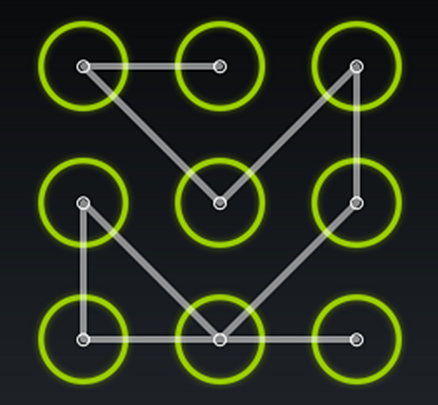
\includegraphics[width=0.2\textwidth]{trace.png} % <- formatos PNG, JPG e PDF
	\small
	\caption[Uso de senha por reconhecimento de padrão]{Uso de senha por reconhecimento de padrão nos \textit{smartphones} Android}
	\label{fig:trace}
\end{figure}